%% ============================================================
%%  Smart Data Warehouse & Agentic NL2SQL System
%%  Full Technical Project Report
%%  Shreya Ghatage · IIT Madras · 22f3000165@ds.study.iitm.ac.in
%% ============================================================
\documentclass[12pt,a4paper]{report}

%% ── Packages ────────────────────────────────────────────────
\usepackage[T1]{fontenc}
\usepackage[utf8]{inputenc}
\usepackage[margin=2.5cm]{geometry}
\usepackage{lmodern}
\usepackage{microtype}
\usepackage{setspace}
\usepackage{titlesec}
\usepackage{titletoc}
\usepackage{tocloft}
\usepackage{fancyhdr}
\usepackage{xcolor}
\usepackage{graphicx}
\usepackage{float}
\usepackage{booktabs}
\usepackage{longtable}
\usepackage{array}
\usepackage{tabularx}
\usepackage{multirow}
\usepackage{enumitem}
\usepackage{listings}
\usepackage{caption}
\usepackage{subcaption}
\usepackage{amsmath}
\usepackage{amssymb}
\usepackage{hyperref}
\usepackage{cleveref}
\usepackage{mdframed}
\usepackage{tcolorbox}
\usepackage{fontawesome5}
\usepackage{tikz}
\usepackage{pgfplots}
\usepackage{adjustbox}
\usepackage{soul}
\usepackage{datetime2}
\usepackage{parskip}
\usetikzlibrary{arrows.meta,shapes,positioning,fit,calc,backgrounds,decorations.pathreplacing}
\pgfplotsset{compat=1.18}

%% ── Colour Palette ──────────────────────────────────────────
\definecolor{DarkBg}{HTML}{080d1a}
\definecolor{AccentBlue}{HTML}{3b82f6}
\definecolor{AccentCyan}{HTML}{06b6d4}
\definecolor{AccentAmber}{HTML}{f59e0b}
\definecolor{AccentGreen}{HTML}{10b981}
\definecolor{AccentRed}{HTML}{ef4444}
\definecolor{SlateLight}{HTML}{94a3b8}
\definecolor{SlateDark}{HTML}{475569}
\definecolor{CodeBg}{HTML}{0f172a}
\definecolor{CodeFg}{HTML}{e2e8f0}

%% ── Hyperref Setup ──────────────────────────────────────────
\hypersetup{
  colorlinks=true,
  linkcolor=AccentBlue,
  citecolor=AccentCyan,
  urlcolor=AccentCyan,
  pdftitle={Smart Data Warehouse \& Agentic NL2SQL System},
  pdfauthor={Shreya Ghatage},
}

%% ── Section Styling ─────────────────────────────────────────
\titleformat{\chapter}[block]
  {\normalfont\Huge\bfseries\color{AccentBlue}}
  {\thechapter.}{12pt}{}
\titleformat{\section}[block]
  {\normalfont\Large\bfseries\color{AccentBlue!85!black}}
  {\thesection}{10pt}{}
\titleformat{\subsection}[block]
  {\normalfont\large\bfseries\color{AccentCyan!80!black}}
  {\thesubsection}{8pt}{}
\titleformat{\subsubsection}[block]
  {\normalfont\normalsize\bfseries\color{SlateDark}}
  {\thesubsubsection}{6pt}{}
\titlespacing*{\chapter}{0pt}{-10pt}{20pt}

%% ── Page Style ───────────────────────────────────────────────
\pagestyle{fancy}
\fancyhf{}
\fancyhead[L]{\small\color{SlateDark}\textit{Smart Data Warehouse \& Agentic NL2SQL}}
\fancyhead[R]{\small\color{SlateDark}Shreya Ghatage}
\fancyfoot[C]{\small\thepage}
\renewcommand{\headrulewidth}{0.4pt}
\renewcommand{\headrule}{\color{AccentBlue!40}\hrule width\headwidth height\headrulewidth}

%% ── Code Listings ────────────────────────────────────────────
\lstdefinestyle{pycode}{
  language=Python,
  backgroundcolor=\color{CodeBg},
  basicstyle=\ttfamily\footnotesize\color{CodeFg},
  keywordstyle=\color{AccentCyan}\bfseries,
  stringstyle=\color{AccentGreen},
  commentstyle=\color{SlateDark}\itshape,
  numberstyle=\tiny\color{SlateDark},
  numbers=left,
  numbersep=8pt,
  breaklines=true,
  breakatwhitespace=true,
  showstringspaces=false,
  frame=single,
  framecolor=AccentBlue!30,
  rulecolor=\color{AccentBlue!30},
  captionpos=b,
  tabsize=4,
  morekeywords={dict,list,str,int,bool,None,True,False,Optional,Callable,dataclass,field},
}
\lstdefinestyle{sqlcode}{
  language=SQL,
  backgroundcolor=\color{CodeBg},
  basicstyle=\ttfamily\footnotesize\color{CodeFg},
  keywordstyle=\color{AccentAmber}\bfseries,
  stringstyle=\color{AccentGreen},
  commentstyle=\color{SlateDark}\itshape,
  numberstyle=\tiny\color{SlateDark},
  numbers=left,
  numbersep=8pt,
  breaklines=true,
  showstringspaces=false,
  frame=single,
  framecolor=AccentBlue!30,
  rulecolor=\color{AccentBlue!30},
  captionpos=b,
  tabsize=4,
}
\lstset{style=pycode}

%% ── Custom Boxes ─────────────────────────────────────────────
\tcbuselibrary{skins,breakable}
\newenvironment{infobox}[1]{%
  \begin{tcolorbox}[enhanced,breakable,
    colback=AccentBlue!8,colframe=AccentBlue!50,
    title={\faInfoCircle\quad#1},
    fonttitle=\bfseries\small\color{AccentBlue},
    coltitle=AccentBlue,
    boxrule=0.6pt,arc=4pt]
}{\end{tcolorbox}}

\newenvironment{bugbox}[1]{%
  \begin{tcolorbox}[enhanced,breakable,
    colback=AccentRed!8,colframe=AccentRed!50,
    title={\faBug\quad#1},
    fonttitle=\bfseries\small\color{AccentRed},
    coltitle=AccentRed,
    boxrule=0.6pt,arc=4pt]
}{\end{tcolorbox}}

\newenvironment{featurebox}[1]{%
  \begin{tcolorbox}[enhanced,breakable,
    colback=AccentGreen!8,colframe=AccentGreen!50,
    title={\faRocket\quad#1},
    fonttitle=\bfseries\small\color{AccentGreen},
    coltitle=AccentGreen,
    boxrule=0.6pt,arc=4pt]
}{\end{tcolorbox}}

%% ── Spacing ──────────────────────────────────────────────────
\setstretch{1.25}
\setlength{\parindent}{0pt}
\setlength{\parskip}{6pt}

%% ─────────────────────────────────────────────────────────────
\begin{document}

%% ══════════════════════════════════════════════════════════════
%%  TITLE PAGE
%% ══════════════════════════════════════════════════════════════
\begin{titlepage}
  \centering
  \vspace*{2cm}
  {\Huge\bfseries\color{AccentBlue}
    Smart Data Warehouse \&\\[6pt]
    Agentic NL2SQL System\\[10pt]}
  {\large\color{AccentCyan} Full Technical Project Report}

  \vspace{1.5cm}
  \rule{0.7\linewidth}{1.5pt}
  \vspace{1cm}

  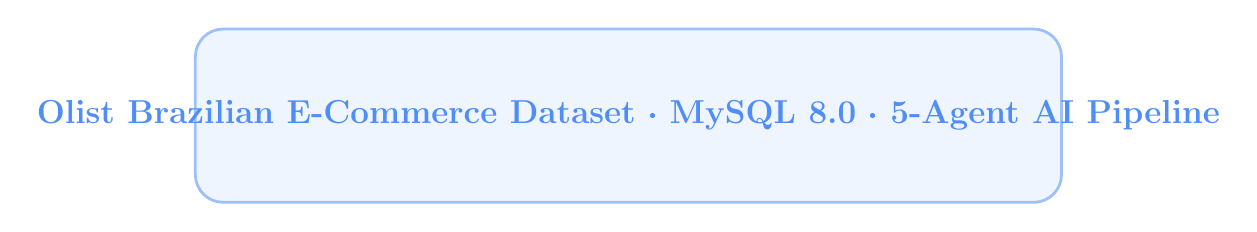
\begin{tikzpicture}
    \node[draw=AccentBlue!50, fill=AccentBlue!8, rounded corners=10pt,
          minimum width=11cm, minimum height=2.2cm, line width=1pt] (box) {};
    \node[font=\large\bfseries, text=AccentBlue!90] at (box) {
      Olist Brazilian E-Commerce Dataset · MySQL 8.0 · 5-Agent AI Pipeline
    };
  \end{tikzpicture}

  \vspace{1.5cm}
  {\large\bfseries Shreya Ghatage}\\[4pt]
  {\normalsize\color{SlateDark} IIT Madras — Data Science Programme}\\
  {\normalsize\color{SlateDark} \texttt{22f3000165@ds.study.iitm.ac.in}}

  \vspace{1.2cm}
  \rule{0.4\linewidth}{0.6pt}
  \vspace{0.8cm}

  \begin{tabular}{rl}
    \textbf{Repository:} & \texttt{github.com/Shreya75/smart-dw-nl2sql}\\[4pt]
    \textbf{Branch:}     & \texttt{develop}\\[4pt]
    \textbf{Commits:}    & 15 (spanning full development arc)\\[4pt]
    \textbf{Date:}       & June 2026\\
  \end{tabular}

  \vfill
  {\small\color{SlateDark}
    Built with Python 3.11 · MySQL 8.0 · Ollama · Groq · Streamlit · Plotly · FastAPI}
\end{titlepage}

%% ══════════════════════════════════════════════════════════════
%%  ABSTRACT
%% ══════════════════════════════════════════════════════════════
\chapter*{Abstract}
\addcontentsline{toc}{chapter}{Abstract}

This report documents the complete end-to-end development of the \textbf{Smart Data Warehouse
NL2SQL System} — an agentic artificial intelligence platform that converts natural-language
business questions into executable SQL, runs them against a production-grade MySQL 8.0
star-schema data warehouse, and returns interactive charts alongside LLM-generated business
insights.

The project is built on the \textbf{Olist Brazilian E-Commerce} dataset (2016--2018), comprising
99,441 orders across 27 states and nine raw CSV files totalling several hundred thousand records.
A production-grade ETL pipeline transforms the raw data into a Kimball-style star schema with one
fact table (\texttt{fact\_sales}) and four dimension tables, incorporating seven derived features
including delivery time, delay days, and a binary late-delivery flag.

The AI core is a \textbf{five-agent sequential pipeline} evolved into a \textbf{ReAct-style
agentic loop}: Agent~1 parses intent, Agent~2 generates SQL, Agent~3 validates safety and schema
correctness, Agent~4 executes against MySQL, and Agent~5 generates business insights. A dedicated
\textbf{Reflection Agent} classifies failures, diagnoses root causes, and plans targeted recovery
strategies between attempts — replacing raw error passthrough with structured reasoning.

The user-facing Streamlit application provides four pages (Query, Dashboard, History, Admin),
supplemented by ten major feature upgrades: multi-turn conversational memory, Brazil geospatial
bubble maps, time-series forecasting, PDF report export, a FastAPI REST endpoint, RFM customer
segmentation, confidence scoring, semantic query caching, voice input, and multi-LLM benchmarking.

The project demonstrates a complete data engineering lifecycle — from raw CSV ingestion through
multi-layer cleaning, star-schema warehousing, agentic AI, and a polished product-quality UI —
in approximately 4,000 lines of Python across 30+ modules.

\tableofcontents
\listoftables

%% ══════════════════════════════════════════════════════════════
\chapter{Introduction}
%% ══════════════════════════════════════════════════════════════

\section{Problem Statement}

Business users need answers from data warehouses but lack SQL expertise. Traditional BI tools
require either pre-built dashboards (inflexible) or direct SQL access (inaccessible). Large
Language Models (LLMs) can generate SQL from natural language, but naive single-LLM approaches
suffer from hallucination, schema mismatch, and unsafe queries.

\textbf{The core challenge:} Build a system that is simultaneously \emph{accurate} (generates
correct SQL for a specific schema), \emph{safe} (never executes destructive statements),
\emph{robust} (recovers from LLM errors automatically), and \emph{accessible} (usable by
non-technical stakeholders via a polished web interface).

\section{Project Objectives}

\begin{enumerate}[leftmargin=*]
  \item Design and populate a production-grade MySQL star-schema warehouse from the Olist
        Brazilian E-Commerce dataset.
  \item Build a multi-agent NL2SQL pipeline with at least five specialised agents.
  \item Evolve the pipeline into a genuine \emph{agentic loop} using the ReAct pattern with
        failure reflection and intent revision.
  \item Deliver a polished multi-page Streamlit UI with real-time charts, AI insights, and
        query history.
  \item Expose the pipeline as a documented REST API.
  \item Add at least ten advanced features that demonstrate data science, ML, and product
        engineering depth.
\end{enumerate}

\section{Significance}

This project sits at the intersection of three currently active research and engineering areas:
\textbf{Text-to-SQL} (NL2SQL), \textbf{agentic AI systems} (multi-step LLM orchestration with
tool use and self-correction), and \textbf{analytical data warehousing} (Kimball star schema,
ETL, performance indexing). The combination produces a system that is both academically grounded
and production-realistic.

\section{Report Structure}

Chapter~\ref{ch:dataset} describes the Olist dataset.
Chapter~\ref{ch:architecture} presents the overall system architecture.
Chapter~\ref{ch:database} details the star-schema design.
Chapter~\ref{ch:etl} documents the ETL pipeline.
Chapter~\ref{ch:agents} explains all five agents and the agentic loop.
Chapter~\ref{ch:ui} covers the Streamlit UI.
Chapter~\ref{ch:features} documents the ten advanced features.
Chapter~\ref{ch:testing} presents the test suite.
Chapter~\ref{ch:history} traces the commit-level development history.
Chapter~\ref{ch:challenges} discusses technical challenges and their solutions.
Chapter~\ref{ch:conclusion} concludes with findings and future work.

%% ══════════════════════════════════════════════════════════════
\chapter{Dataset: Olist Brazilian E-Commerce}
\label{ch:dataset}
%% ══════════════════════════════════════════════════════════════

\section{Overview}

The Olist dataset is a publicly available real-world e-commerce dataset from Brazil's largest
online marketplace. It covers orders placed between September 2016 and October 2018 and is
released under a Creative Commons licence. The dataset was obtained from Kaggle.

\begin{table}[H]
  \centering
  \caption{Raw CSV files in the Olist dataset}
  \label{tab:raw-files}
  \renewcommand{\arraystretch}{1.3}
  \begin{tabularx}{\textwidth}{lXr}
    \toprule
    \textbf{File} & \textbf{Contents} & \textbf{Rows} \\
    \midrule
    \texttt{olist\_orders\_dataset.csv}         & Order headers: status, timestamps & 99,441 \\
    \texttt{olist\_order\_items\_dataset.csv}   & Per-item price, freight, seller & 112,650 \\
    \texttt{olist\_order\_payments\_dataset.csv}& Payment type, instalment, value & 103,886 \\
    \texttt{olist\_order\_reviews\_dataset.csv} & Customer review scores \& text  & 99,224 \\
    \texttt{olist\_customers\_dataset.csv}      & Customer city, state, zip code  & 99,441 \\
    \texttt{olist\_sellers\_dataset.csv}        & Seller city, state, zip code    & 3,095 \\
    \texttt{olist\_products\_dataset.csv}       & Category, dimensions, weight    & 32,951 \\
    \texttt{olist\_geolocation\_dataset.csv}    & Zip → lat/lon mappings          & 1,000,163 \\
    \texttt{product\_category\_name\_translation.csv} & Portuguese→English labels & 71 \\
    \bottomrule
  \end{tabularx}
\end{table}

\section{Key Metrics}

After ETL processing and warehousing (delivered orders only):

\begin{table}[H]
  \centering
  \caption{Warehouse KPI snapshot — delivered orders}
  \label{tab:kpis}
  \renewcommand{\arraystretch}{1.3}
  \begin{tabular}{ll}
    \toprule
    \textbf{Metric} & \textbf{Value} \\
    \midrule
    Total delivered orders       & $\sim$96,000 \\
    Total revenue (payment\_value) & R\$\,16.0M+ \\
    Unique customers             & $\sim$96,000 \\
    Unique sellers               & 3,095 \\
    Product categories (English) & 74 \\
    Brazilian states covered     & 27 \\
    Date range                   & Sept 2016 -- Oct 2018 \\
    Average review score         & 4.07 / 5 \\
    Average delivery time        & $\sim$12 days \\
    Late delivery rate           & $\sim$7\% \\
    \bottomrule
  \end{tabular}
\end{table}

\section{Data Quality Issues Encountered}

\begin{itemize}[leftmargin=*]
  \item \textbf{Typos in column names}: \texttt{product\_name\_lenght} $\to$
        \texttt{product\_name\_length} (corrected in cleaning).
  \item \textbf{Missing categories}: $\sim$610 products had no Portuguese category name;
        filled as \texttt{"unknown"} post-merge.
  \item \textbf{Null timestamps}: Orders with null \texttt{order\_delivered\_customer\_date}
        produce NaN delivery times; handled with \texttt{pd.to\_datetime(errors="coerce")}.
  \item \textbf{Duplicate payments}: Some orders had multiple payment records (instalment rows);
        aggregated to primary type and total value at order level.
  \item \textbf{Geolocation}: Not used in the warehouse (duplicate data); excluded from ETL.
\end{itemize}

%% ══════════════════════════════════════════════════════════════
\chapter{System Architecture}
\label{ch:architecture}
%% ══════════════════════════════════════════════════════════════

\section{High-Level Design}

The system follows a layered architecture with four distinct tiers:

\begin{figure}[H]
  \centering
  \begin{tikzpicture}[
    box/.style={draw=AccentBlue!50, fill=AccentBlue!8, rounded corners=8pt,
                minimum width=9cm, minimum height=1.1cm, text=AccentBlue!90,
                font=\bfseries\small, line width=0.8pt},
    arrow/.style={-{Stealth[length=6pt]}, AccentBlue!60, line width=1pt},
  ]
    \node[box] (ui)   at (0, 6)   {\faDesktop\quad Streamlit Multi-Page UI (4 pages + FastAPI)};
    \node[box] (pipe) at (0, 4.2) {\faRobot\quad 5-Agent NL2SQL Pipeline + Reflection Agent};
    \node[box] (exec) at (0, 2.4) {\faDatabase\quad SQL Validation + MySQL Execution Engine};
    \node[box] (dw)   at (0, 0.6) {\faWarehouse\quad MySQL 8.0 Star-Schema Warehouse (5 tables)};
    \node[box, fill=AccentCyan!8, draw=AccentCyan!50, text=AccentCyan!80]
              (etl)  at (0,-1.2) {\faArrowRight\quad ETL Pipeline · Olist CSVs $\to$ Warehouse};
    \draw[arrow] (ui)   -- (pipe);
    \draw[arrow] (pipe) -- (exec);
    \draw[arrow] (exec) -- (dw);
    \draw[arrow] (etl)  -- (dw);
    \node[right=0.5cm of ui,   font=\tiny\color{SlateDark}] {Chapters 7};
    \node[right=0.5cm of pipe, font=\tiny\color{SlateDark}] {Chapter 5};
    \node[right=0.5cm of exec, font=\tiny\color{SlateDark}] {Chapter 5};
    \node[right=0.5cm of dw,   font=\tiny\color{SlateDark}] {Chapter 4};
    \node[right=0.5cm of etl,  font=\tiny\color{SlateDark}] {Chapter 6};
  \end{tikzpicture}
  \caption{Four-tier system architecture}
  \label{fig:architecture}
\end{figure}

\section{Technology Stack}

\begin{table}[H]
  \centering
  \caption{Full technology stack}
  \label{tab:stack}
  \renewcommand{\arraystretch}{1.3}
  \begin{tabularx}{\textwidth}{llX}
    \toprule
    \textbf{Layer} & \textbf{Technology} & \textbf{Purpose} \\
    \midrule
    LLM (local)   & Ollama + Llama~3 / Mistral & Private, zero-cost inference \\
    LLM (cloud)   & Groq API + llama3-70b       & Fast cloud inference (free tier) \\
    Database       & MySQL 8.0                   & Star-schema warehouse \\
    ORM / SQL      & SQLAlchemy 2.0 + PyMySQL    & Connection pooling, safe query execution \\
    Data wrangling & Pandas 2.2 + NumPy 1.26     & ETL transformations, feature engineering \\
    Web UI         & Streamlit 1.35              & Multi-page interactive app \\
    REST API       & FastAPI + Uvicorn           & Programmatic pipeline access \\
    Charts         & Plotly 5.22                 & Interactive visualisations \\
    ML             & scikit-learn                & Forecasting, RFM clustering \\
    Validation     & sqlparse 0.5 + regex        & SQL safety checks \\
    Retry          & tenacity 3.x                & Exponential-backoff DB retries \\
    Logging        & loguru 0.7                  & Structured JSONL query log \\
    PDF export     & fpdf2                       & Branded PDF report generation \\
    Similarity     & sklearn TF-IDF              & Semantic query cache \\
    Testing        & pytest 8.2 + pytest-cov     & Unit + integration test suite \\
    \bottomrule
  \end{tabularx}
\end{table}

\section{Project Directory Structure}

\begin{lstlisting}[style=sqlcode, caption={Full project directory layout}, label={lst:tree}]
Final_Project/
 agents/              # The 5 NL2SQL agents + pipeline orchestrator
   query_agent.py     # Agent 1: NL -> intent JSON
   sql_agent.py       # Agent 2: intent -> SQL
   validation_agent.py# Agent 3: safety + schema checks
   execution_agent.py # Agent 4: MySQL execution
   insight_agent.py   # Agent 5: LLM business insights
   pipeline.py        # Orchestrator: ReAct agentic loop
   reflection_agent.py# Error classifier + recovery planner
 analytics/           # Advanced analytics modules
   forecasting.py     # Ridge regression time-series forecasting
   rfm.py             # RFM segmentation with KMeans
 api/
   main.py            # FastAPI REST endpoint (/query, /health, /schema)
 app/
   Home.py            # Landing page with live KPIs
   components/
     chart_builder.py # Smart adaptive chart selection
     conversation.py  # Multi-turn memory manager
     insight_display.py # 4-card AI insight renderer
     styles.py        # Global CSS + Plotly theme
   pages/
     1_Query.py       # NL query page (voice, cache, benchmarking)
     2_Dashboard.py   # 9-section KPI dashboard
     3_History.py     # Persistent query log browser
     4_Admin.py       # DB status, schema explorer, diagnostics
 data/raw/            # 9 Olist CSV files
 database/
   schema.sql         # Star-schema DDL
   sample_queries.sql # 20 benchmark analytical queries
 etl/
   data_ingestion.py  # CSV file readers
   data_cleaning.py   # Dedup, type coercion, normalisation
   data_integration.py# Cross-table join and merge
   feature_engineering.py # Delivery time, delay, is_late, approval hours
   data_loading.py    # Dim + fact table writers with FK-safe truncate
 tests/               # pytest test suite (54 tests)
 utils/
   confidence.py      # 0-100 pipeline confidence scorer
   db_connection.py   # SQLAlchemy engine singleton
   llm_client.py      # Unified Ollama/Groq dispatcher
   logger.py          # loguru setup
   query_cache.py     # TF-IDF semantic cache
   report_generator.py# fpdf2 PDF report builder
 config.py            # .env-backed configuration
 requirements.txt     # Pinned dependencies
 run_etl.py           # ETL entry point
\end{lstlisting}

%% ══════════════════════════════════════════════════════════════
\chapter{Database Design: Star Schema}
\label{ch:database}
%% ══════════════════════════════════════════════════════════════

\section{Design Philosophy}

The warehouse follows the \textbf{Kimball Dimensional Modelling} approach: a central fact table
recording transactional events, surrounded by denormalised dimension tables. This design optimises
for analytical queries (GROUP BY, aggregations, date-range slices) at the expense of write
normalisation — appropriate for a read-heavy analytical workload.

\section{Entity-Relationship Diagram}

\begin{figure}[H]
  \centering
  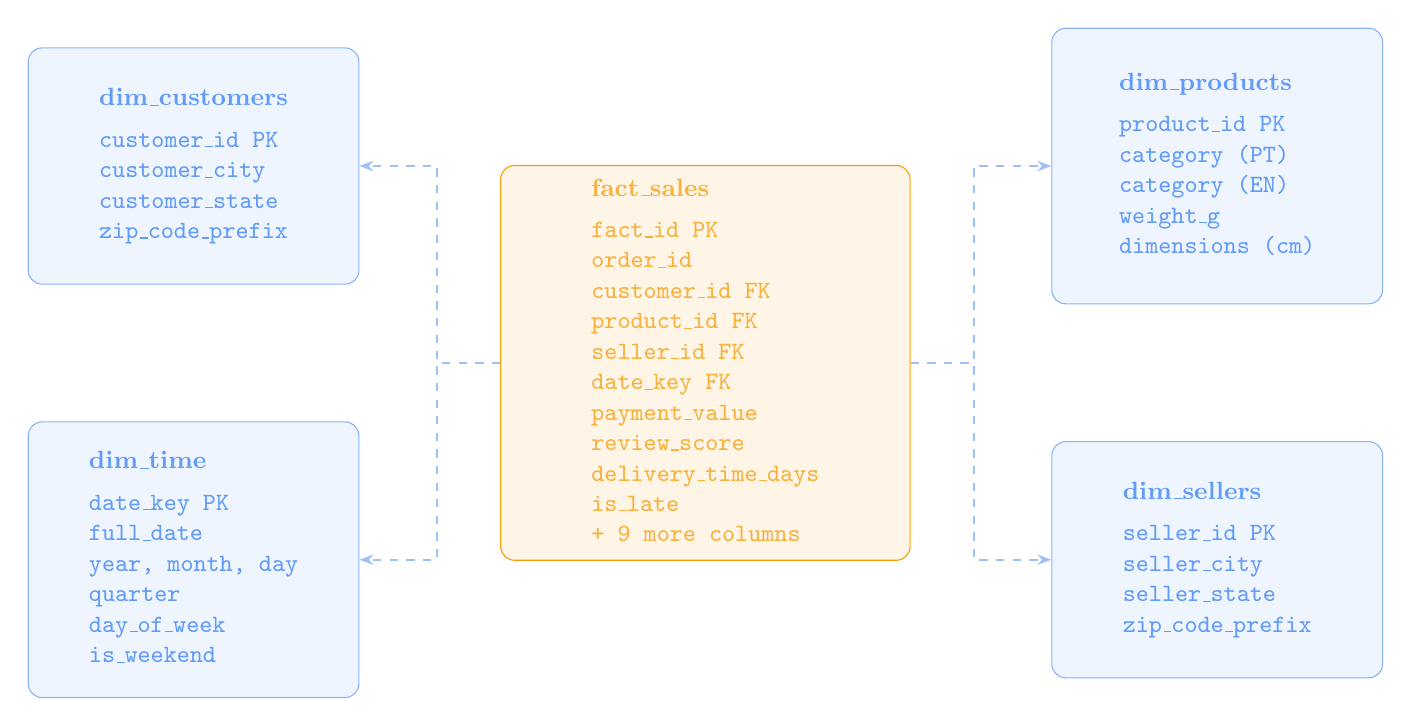
\begin{tikzpicture}[
    fact/.style={draw=AccentAmber, fill=AccentAmber!10, rounded corners=5pt,
                 minimum width=5.2cm, font=\small\bfseries, text=AccentAmber!80},
    dim/.style={draw=AccentBlue!60, fill=AccentBlue!8, rounded corners=5pt,
                minimum width=4.2cm, font=\small\bfseries, text=AccentBlue!80},
    fk/.style={-{Stealth[length=5pt]}, AccentBlue!50, dashed, line width=0.8pt},
  ]
    % Fact table
    \node[fact, minimum height=5cm] (fact) at (0,0) {
      \begin{tabular}{l}
        \textbf{fact\_sales}\\[4pt]
        \texttt{\small fact\_id PK}\\
        \texttt{\small order\_id}\\
        \texttt{\small customer\_id FK}\\
        \texttt{\small product\_id FK}\\
        \texttt{\small seller\_id FK}\\
        \texttt{\small date\_key FK}\\
        \texttt{\small payment\_value}\\
        \texttt{\small review\_score}\\
        \texttt{\small delivery\_time\_days}\\
        \texttt{\small is\_late}\\
        \texttt{\small + 9 more columns}
      \end{tabular}
    };
    % dim_customers
    \node[dim, minimum height=3cm] (dc) at (-6.5, 2.5) {
      \begin{tabular}{l}
        \textbf{dim\_customers}\\[4pt]
        \texttt{\small customer\_id PK}\\
        \texttt{\small customer\_city}\\
        \texttt{\small customer\_state}\\
        \texttt{\small zip\_code\_prefix}
      \end{tabular}
    };
    % dim_products
    \node[dim, minimum height=3.5cm] (dp) at (6.5, 2.5) {
      \begin{tabular}{l}
        \textbf{dim\_products}\\[4pt]
        \texttt{\small product\_id PK}\\
        \texttt{\small category (PT)}\\
        \texttt{\small category (EN)}\\
        \texttt{\small weight\_g}\\
        \texttt{\small dimensions (cm)}
      \end{tabular}
    };
    % dim_sellers
    \node[dim, minimum height=3cm] (ds) at (6.5, -2.5) {
      \begin{tabular}{l}
        \textbf{dim\_sellers}\\[4pt]
        \texttt{\small seller\_id PK}\\
        \texttt{\small seller\_city}\\
        \texttt{\small seller\_state}\\
        \texttt{\small zip\_code\_prefix}
      \end{tabular}
    };
    % dim_time
    \node[dim, minimum height=3.5cm] (dt) at (-6.5, -2.5) {
      \begin{tabular}{l}
        \textbf{dim\_time}\\[4pt]
        \texttt{\small date\_key PK}\\
        \texttt{\small full\_date}\\
        \texttt{\small year, month, day}\\
        \texttt{\small quarter}\\
        \texttt{\small day\_of\_week}\\
        \texttt{\small is\_weekend}
      \end{tabular}
    };
    % FK arrows
    \draw[fk] (fact.west) -- +(-0.8,0) |- (dc.east);
    \draw[fk] (fact.east) -- +(0.8,0)  |- (dp.west);
    \draw[fk] (fact.east) -- +(0.8,0)  |- (ds.west);
    \draw[fk] (fact.west) -- +(-0.8,0) |- (dt.east);
  \end{tikzpicture}
  \caption{Star schema entity-relationship diagram}
  \label{fig:erd}
\end{figure}

\section{Table Definitions}

\subsection{Fact Table: \texttt{fact\_sales}}

The fact table stores one row per order-item (an order with two items creates two rows). It
records all measurable business events.

\begin{lstlisting}[style=sqlcode, caption={fact\_sales DDL excerpt}, label={lst:fact}]
CREATE TABLE fact_sales (
  fact_id              BIGINT AUTO_INCREMENT PRIMARY KEY,
  order_id             VARCHAR(36) NOT NULL,
  order_item_id        INT,
  customer_id          VARCHAR(36),   -- FK → dim_customers
  product_id           VARCHAR(36),   -- FK → dim_products
  seller_id            VARCHAR(36),   -- FK → dim_sellers
  date_key             INT,           -- FK → dim_time (YYYYMMDD)
  order_status         VARCHAR(20),
  payment_type         VARCHAR(20),
  payment_value        DECIMAL(10,2),
  price                DECIMAL(10,2),
  freight_value        DECIMAL(10,2),
  review_score         TINYINT,
  delivery_time_days   DECIMAL(6,2),  -- DERIVED feature
  delay_days           DECIMAL(6,2),  -- DERIVED: positive = late
  is_late              TINYINT(1),    -- DERIVED binary flag
  approval_time_hours  DECIMAL(8,2),  -- DERIVED feature
  ...
) ENGINE=InnoDB DEFAULT CHARSET=utf8mb4;
\end{lstlisting}

\subsection{Dimension Tables}

\begin{table}[H]
  \centering
  \caption{Dimension table summary}
  \label{tab:dims}
  \renewcommand{\arraystretch}{1.3}
  \begin{tabularx}{\textwidth}{lXrr}
    \toprule
    \textbf{Table} & \textbf{Purpose} & \textbf{Rows} & \textbf{Key columns} \\
    \midrule
    \texttt{dim\_time}      & Calendar dimension, date attributes & $\sim$750 & year, month, quarter, day\_of\_week \\
    \texttt{dim\_customers} & Customer geography                  & 99,441    & state, city \\
    \texttt{dim\_products}  & Product attributes + English category & 32,951  & category\_name\_english \\
    \texttt{dim\_sellers}   & Seller geography                    & 3,095     & seller\_state, seller\_city \\
    \bottomrule
  \end{tabularx}
\end{table}

\section{Indexing Strategy}

MySQL 8.0 enforces \texttt{ONLY\_FULL\_GROUP\_BY} mode, meaning every non-aggregated SELECT
column must appear in GROUP BY. This influenced both index design and the SQL generation
prompts. Composite indexes were chosen to support the most common analytical patterns:

\begin{lstlisting}[style=sqlcode, caption={Composite indexes on fact\_sales}]
CREATE INDEX idx_fact_date_cust  ON fact_sales(date_key, customer_id);
CREATE INDEX idx_fact_product    ON fact_sales(product_id, payment_value);
CREATE INDEX idx_fact_seller     ON fact_sales(seller_id, review_score);
CREATE INDEX idx_time_year_month ON dim_time(year, month);
CREATE INDEX idx_cust_state_city ON dim_customers(customer_state, customer_city);
\end{lstlisting}

%% ══════════════════════════════════════════════════════════════
\chapter{ETL Pipeline}
\label{ch:etl}
%% ══════════════════════════════════════════════════════════════

\section{Pipeline Stages}

The ETL pipeline consists of five sequential stages, each implemented as a dedicated Python
module under the \texttt{etl/} directory.

\begin{figure}[H]
  \centering
  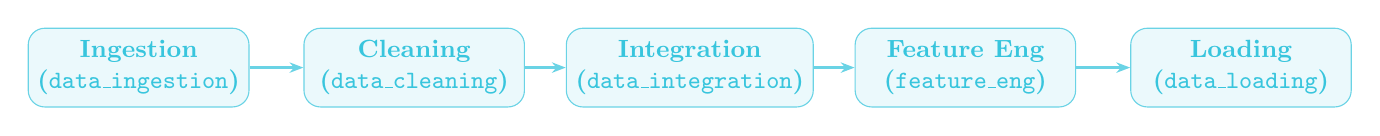
\begin{tikzpicture}[
    stage/.style={draw=AccentCyan!60, fill=AccentCyan!8, rounded corners=6pt,
                  minimum width=2.8cm, minimum height=1cm, font=\small\bfseries,
                  text=AccentCyan!80, align=center},
    arrow/.style={-{Stealth[length=5pt]}, AccentCyan!60, line width=1pt},
  ]
    \node[stage] (ing)  at (0,0)    {Ingestion\\(\texttt{data\_ingestion})};
    \node[stage] (cln)  at (3.5,0)  {Cleaning\\(\texttt{data\_cleaning})};
    \node[stage] (int)  at (7,0)    {Integration\\(\texttt{data\_integration})};
    \node[stage] (feat) at (10.5,0) {Feature Eng\\(\texttt{feature\_eng})};
    \node[stage] (load) at (14,0)   {Loading\\(\texttt{data\_loading})};
    \draw[arrow] (ing)  -- (cln);
    \draw[arrow] (cln)  -- (int);
    \draw[arrow] (int)  -- (feat);
    \draw[arrow] (feat) -- (load);
  \end{tikzpicture}
  \caption{Five-stage ETL pipeline}
  \label{fig:etl}
\end{figure}

\subsection{Stage 1 — Ingestion (\texttt{data\_ingestion.py})}

Reads all nine raw CSV files from \texttt{data/raw/} using \texttt{pd.read\_csv()} with
appropriate \texttt{dtype} hints. Returns a dictionary keyed by table name.

\subsection{Stage 2 — Cleaning (\texttt{data\_cleaning.py})}

Per-table cleaning functions handle:
\begin{itemize}
  \item \textbf{Deduplication}: \texttt{drop\_duplicates(subset=[primary\_key])}
  \item \textbf{Datetime parsing}: \texttt{pd.to\_datetime(errors="coerce")} for 7 timestamp columns
  \item \textbf{String normalisation}: city names lowercased, states uppercased
  \item \textbf{Numeric coercion}: \texttt{pd.to\_numeric(errors="coerce")} with median imputation
  \item \textbf{Column rename}: Fixes Olist typos (\texttt{lenght} $\to$ \texttt{length})
  \item \textbf{Category translation}: Merges Portuguese$\to$English lookup table
\end{itemize}

\subsection{Stage 3 — Integration (\texttt{data\_integration.py})}

Joins orders with customers, products, items, payments, and reviews at the order level.
Critical design choice: payments are aggregated to \emph{order-level} totals because Olist
records instalment payments as separate rows.

\subsection{Stage 4 — Feature Engineering (\texttt{feature\_engineering.py})}

Derives four business-critical features from timestamp arithmetic:

\begin{lstlisting}[caption={Derived feature computation}]
df["delivery_time_days"] = (
    (df["order_delivered_customer_date"]
     - df["order_purchase_timestamp"])
    .dt.total_seconds() / 86400
).round(2)

df["delay_days"] = (
    (df["order_delivered_customer_date"]
     - df["order_estimated_delivery_date"])
    .dt.total_seconds() / 86400
).round(2)                  # positive = late, negative = early

df["is_late"]   = (df["delay_days"] > 0).astype(int)

df["approval_time_hours"] = (
    (df["order_approved_at"]
     - df["order_purchase_timestamp"])
    .dt.total_seconds() / 3600
).round(2)
\end{lstlisting}

\subsection{Stage 5 — Loading (\texttt{data\_loading.py})}

Writes dimensions and facts to MySQL using \texttt{DataFrame.to\_sql(if\_exists="append")}.
A critical design decision addressed an early ETL bug:

\begin{bugbox}{FK Constraint Violation on Re-run}
  On the second ETL run, \texttt{if\_exists="replace"} dropped and recreated tables,
  violating foreign key constraints. The fix was to disable FK checks, truncate all tables
  in fact-first order, then re-enable FK checks before inserting:
  \begin{lstlisting}[style=sqlcode]
conn.execute(text("SET FOREIGN_KEY_CHECKS=0"))
for t in ["fact_sales","dim_customers","dim_products","dim_sellers","dim_time"]:
    conn.execute(text(f"TRUNCATE TABLE {t}"))
conn.execute(text("SET FOREIGN_KEY_CHECKS=1"))
  \end{lstlisting}
\end{bugbox}

%% ══════════════════════════════════════════════════════════════
\chapter{Multi-Agent NL2SQL Pipeline}
\label{ch:agents}
%% ══════════════════════════════════════════════════════════════

\section{Design Philosophy}

The pipeline implements the principle of \textbf{separation of concerns}: each agent has
exactly one responsibility, receives a typed input, and returns a typed output. No agent knows
about agents that come after it. The pipeline orchestrator is the only component that sees the
full state.

\section{Agent 1 — Query Understanding}

\textbf{Input}: Raw natural-language question (string)\\
\textbf{Output}: Structured JSON intent dict

Agent~1 sends the user question to the LLM with a detailed system prompt specifying the exact
JSON schema to produce. The schema encodes all information needed by Agent~2 to construct a
valid SQL query:

\begin{lstlisting}[caption={Intent JSON schema}]
{
  "intent":    "aggregation | trend | comparison | lookup | ranking",
  "metric":    "revenue | orders | review_score | delivery_time_days | ...",
  "dimension": "customer_state | product_category_name_english | ...",
  "filters":   {"year": 2018, "order_status": "delivered", ...},
  "limit":     5,
  "sort_order": "DESC",
  "time_grain": "monthly | quarterly | annual | null"
}
\end{lstlisting}

\textbf{Self-check}: After running, the pipeline checks whether both \texttt{metric} and
\texttt{dimension} are absent. If so, Agent~1 is re-run with a clarification nudge — the
first example of intent validation in the agentic loop.

\section{Agent 2 — NL2SQL Generation}

\textbf{Input}: Intent JSON + original question + (optional) reflection feedback\\
\textbf{Output}: Raw MySQL SELECT statement

Agent~2 receives the full schema context (all five tables with column types and join conditions)
and a critical system prompt that explicitly enforces MySQL~8.0's \texttt{ONLY\_FULL\_GROUP\_BY}
rules with WRONG/CORRECT examples:

\begin{lstlisting}[style=sqlcode, caption={ONLY\_FULL\_GROUP\_BY enforcement in prompt}]
-- WRONG (will always fail on MySQL 8.0):
SELECT dt.full_date, SUM(fs.payment_value) AS revenue
FROM fact_sales fs JOIN dim_time dt ON fs.date_key=dt.date_key
GROUP BY YEAR(dt.full_date), MONTH(dt.full_date)
-- Error 1055: dt.full_date not in GROUP BY

-- CORRECT pattern:
SELECT dt.year, dt.month,
       CONCAT(dt.year,'-',LPAD(dt.month,2,'0')) AS month_label,
       ROUND(SUM(fs.payment_value),0) AS revenue
FROM fact_sales fs JOIN dim_time dt ON fs.date_key=dt.date_key
GROUP BY dt.year, dt.month
ORDER BY dt.year, dt.month ASC
\end{lstlisting}

\textbf{SQL extraction}: LLMs (especially Mistral) often prepend prose to the SQL. A
two-step extraction pipeline was implemented:

\begin{lstlisting}[caption={SQL extraction from LLM prose output}]
sql = re.sub(r"```(?:sql)?\s*", "", sql, flags=re.IGNORECASE).strip()
m = re.search(r"\bSELECT\b", sql, re.IGNORECASE)
if m:
    sql = sql[m.start():]           # slice from first SELECT
    sql = re.split(r"\n[ \t]*\n", sql)[0]  # stop at first blank line
sql = sql.rstrip(";").strip()
\end{lstlisting}

\section{Agent 3 — SQL Validation}

\textbf{Input}: SQL string\\
\textbf{Output}: \texttt{ValidationResult(is\_valid, errors, warnings)}

This agent is purely rule-based — no LLM call. It enforces:

\begin{enumerate}[leftmargin=*]
  \item \textbf{Forbidden keyword check}: Regex blocks DELETE, DROP, UPDATE, INSERT, TRUNCATE,
        ALTER, EXEC, GRANT, REVOKE, CREATE, REPLACE, CALL, LOAD.
  \item \textbf{SELECT-only check}: Query must begin with SELECT after stripping whitespace.
  \item \textbf{sqlparse syntax}: Verifies the query parses without error.
  \item \textbf{Table allowlist}: Any table name not in \{fact\_sales, dim\_customers,
        dim\_products, dim\_sellers, dim\_time\} generates an error.
  \item \textbf{Complexity warnings}: More than 5 JOINs or 2 subqueries trigger advisory
        warnings (non-blocking).
\end{enumerate}

Rule-based validation is deliberate: LLM-based validation would be slow, expensive, and could
itself hallucinate. The rule-based approach is deterministic, instantaneous, and provably
conservative.

\section{Agent 4 — SQL Execution}

\textbf{Input}: Validated SQL string\\
\textbf{Output}: \texttt{pd.DataFrame} of results

The execution agent runs the SQL with \texttt{tenacity} retry (3 attempts, exponential backoff
with jitter). A per-session timeout is applied before each query:

\begin{lstlisting}[caption={Execution agent with retry and timeout}]
@retry(stop=stop_after_attempt(3),
       wait=wait_exponential(multiplier=1, min=1, max=4),
       retry=retry_if_exception_type(Exception), reraise=True)
def execute_query(sql: str) -> pd.DataFrame:
    with engine.connect() as conn:
        conn.execute(text(f"SET SESSION MAX_EXECUTION_TIME={timeout_ms}"))
        result = conn.execute(text(sql))          # text() prevents % format errors
        return pd.DataFrame(result.fetchall(),
                            columns=list(result.keys()))
\end{lstlisting}

\textbf{Critical detail}: \texttt{sqlalchemy.text()} is mandatory. Without it,
\texttt{pymysql} interprets \texttt{\%Y} and \texttt{\%m} inside SQL strings as Python format
specifiers, causing a \texttt{TypeError} on any query containing date-format functions.

\section{Agent 5 — Insight Generation}

\textbf{Input}: Original question + SQL + top-20 rows of DataFrame (markdown table)\\
\textbf{Output}: Dict with four keys: summary, key\_finding, trend, recommendation

Agent~5 acts as a senior e-commerce business analyst, receiving both the question and the
actual query results. It generates structured JSON with \texttt{temperature=0.3} (slightly
above zero to allow variation while maintaining coherence).

\section{The Pipeline Orchestrator: From Linear to Agentic}
\label{sec:agentic}

\subsection{Original Linear Pipeline (v1)}

The initial implementation was a simple \texttt{for attempt in range(3)} loop:

\begin{lstlisting}[caption={Original sequential pipeline (non-agentic)}]
# Agent 1 runs once, never questioned
result.intent = understand_query(user_query)

error_feedback = ""
for attempt in range(1, MAX_RETRY_ATTEMPTS + 1):
    result.sql = generate_sql(result.intent, user_query, error_feedback)
    result.validation = validate_sql(result.sql)
    if not result.validation.is_valid:
        error_feedback = " | ".join(result.validation.errors)  # raw error passthrough
        continue
    result.data = execute_query(result.sql)
    break
result.insights = generate_insights(...)
\end{lstlisting}

\textbf{Problems identified}:
\begin{enumerate}
  \item Agent~1 runs exactly once; a wrong intent is never corrected.
  \item Raw error strings are passed back to Agent~2 — no reasoning about root cause.
  \item Empty results (0 rows) are silently accepted.
  \item No agent ``observes'' what happened before deciding what to do next.
\end{enumerate}

\subsection{Agentic ReAct Loop (v2)}

The upgraded pipeline implements the \textbf{ReAct} (Reason + Act) pattern. Each iteration
follows: \emph{Observe} current state $\to$ \emph{Reason} via Reflection Agent $\to$
\emph{Act} by deciding next agent to invoke.

\begin{figure}[H]
  \centering
  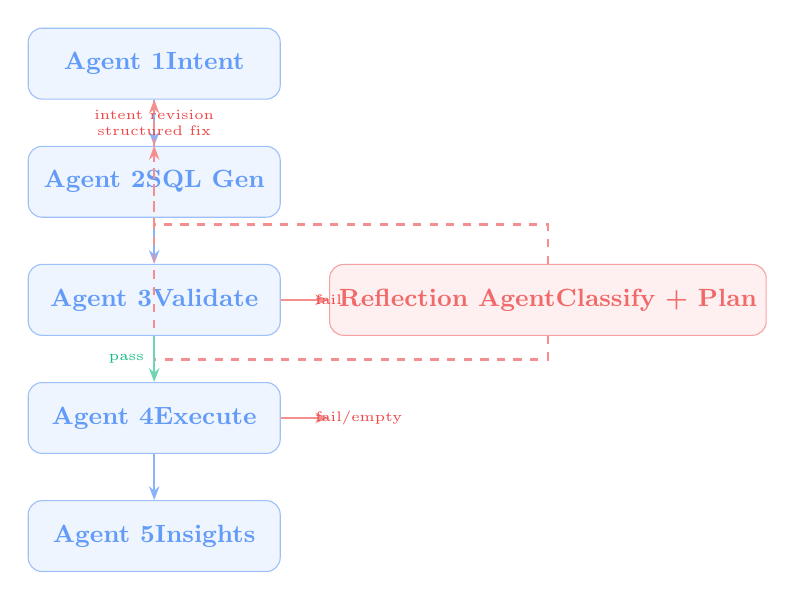
\begin{tikzpicture}[
    agent/.style={draw=AccentBlue!50, fill=AccentBlue!8, rounded corners=5pt,
                  minimum width=3.2cm, minimum height=0.9cm, font=\small\bfseries,
                  text=AccentBlue!80},
    reflect/.style={draw=AccentRed!50, fill=AccentRed!8, rounded corners=5pt,
                    minimum width=3cm, minimum height=0.9cm, font=\small\bfseries,
                    text=AccentRed!80},
    arrow/.style={-{Stealth[length=5pt]}, line width=0.8pt},
    back/.style={-{Stealth[length=5pt]}, AccentRed!60, dashed, line width=0.8pt},
  ]
    \node[agent] (a1) at (0,4)    {Agent 1\\Intent};
    \node[agent] (a2) at (0,2.5)  {Agent 2\\SQL Gen};
    \node[agent] (a3) at (0,1)    {Agent 3\\Validate};
    \node[agent] (a4) at (0,-0.5) {Agent 4\\Execute};
    \node[agent] (a5) at (0,-2)   {Agent 5\\Insights};
    \node[reflect] (rf) at (5,1)  {Reflection Agent\\Classify + Plan};
    \draw[arrow,AccentBlue!60] (a1) -- (a2);
    \draw[arrow,AccentBlue!60] (a2) -- (a3);
    \draw[arrow,AccentBlue!60] (a4) -- (a5);
    \draw[arrow,AccentRed!60]  (a3.east) -- node[right,font=\tiny,color=AccentRed]{fail} (rf.west |- a3);
    \draw[arrow,AccentRed!60]  (a4.east) -- node[right,font=\tiny,color=AccentRed]{fail/empty} (rf.west |- a4);
    \draw[back] (rf.north) -- ++(0,0.5) -| (a2.north) node[above,font=\tiny,color=AccentRed]{structured fix};
    \draw[back] (rf.south) -- ++(0,-0.3) -| (a1.south) node[below,font=\tiny,color=AccentRed]{intent revision};
    \draw[arrow,AccentGreen!60] (a3) -- node[left,font=\tiny,color=AccentGreen]{pass} (a4);
  \end{tikzpicture}
  \caption{ReAct agentic loop with Reflection Agent}
  \label{fig:react}
\end{figure}

\section{The Reflection Agent}

The Reflection Agent is the reasoning layer between attempts. It:

\begin{enumerate}
  \item \textbf{Classifies} the error using fast rule-based regex patterns (8 categories).
  \item \textbf{Plans} a targeted fix using per-category fix instructions.
  \item For \textbf{unknown} errors, invokes the LLM for targeted diagnosis.
  \item Returns a structured dict: \texttt{\{error\_type, root\_cause, fix\_instruction,
        should\_revise\_intent\}}.
\end{enumerate}

\begin{table}[H]
  \centering
  \caption{Reflection Agent error categories and fix strategies}
  \label{tab:errors}
  \renewcommand{\arraystretch}{1.3}
  \begin{tabularx}{\textwidth}{lX}
    \toprule
    \textbf{Error Type} & \textbf{Fix Strategy} \\
    \midrule
    \texttt{group\_by\_violation} & Enforce GROUP BY on all non-aggregate SELECT columns; use \texttt{dt.year}/\texttt{dt.month} not \texttt{YEAR(col)} \\
    \texttt{unknown\_column}      & Replace hallucinated column name with schema-verified equivalent; revise intent \\
    \texttt{syntax\_error}        & Rewrite from scratch; check comma placement, parentheses, JOIN syntax \\
    \texttt{table\_not\_found}    & Replace invalid table with one of the 5 known tables \\
    \texttt{query\_timeout}       & Add \texttt{WHERE order\_status='delivered'} filter; add LIMIT \\
    \texttt{empty\_result}        & Relax date/status filters; broaden WHERE clause \\
    \texttt{validation\_no\_select} & Output bare SQL only — strip all prose and markdown \\
    \texttt{forbidden\_keyword}   & Generate SELECT-only; never use DDL/DML keywords \\
    \bottomrule
  \end{tabularx}
\end{table}

\textbf{Key design decision}: Known error types (7 of 8) use purely rule-based fix instructions
— no LLM call. This keeps the retry latency low. Only genuinely ``unknown'' errors escalate to
an LLM diagnosis call.

\section{Progress Callbacks and Agent Trace}

The pipeline accepts an \texttt{on\_progress} callback that fires after every significant action.
Each event is a dict: \texttt{\{agent, action, message, ...\}}. Events are:
\begin{itemize}
  \item Appended to \texttt{PipelineResult.agent\_trace} (visible in the UI ``Agent Trace'' tab).
  \item Serialised to \texttt{logs/query\_log.jsonl} for audit purposes.
\end{itemize}

%% ══════════════════════════════════════════════════════════════
\chapter{LLM Client}
\label{ch:llm}
%% ══════════════════════════════════════════════════════════════

\section{Unified Provider Abstraction}

All five LLM-calling agents share a single \texttt{utils/llm\_client.py} module. This
abstraction allows switching providers at runtime without changing any agent code:

\begin{lstlisting}[caption={Unified LLM client dispatcher}]
def chat(messages: list[dict], json_mode: bool = False,
         temperature: float = 0) -> str:
    provider, model = get_active_provider()
    if provider == "groq":
        return _groq_chat(messages, model, json_mode, temperature)
    return _ollama_chat(messages, model, json_mode, temperature)
\end{lstlisting}

\section{Provider Comparison}

\begin{table}[H]
  \centering
  \caption{Supported LLM providers}
  \label{tab:providers}
  \renewcommand{\arraystretch}{1.3}
  \begin{tabularx}{\textwidth}{lXXl}
    \toprule
    \textbf{Provider} & \textbf{Models} & \textbf{Characteristics} & \textbf{Cost} \\
    \midrule
    Ollama (local)  & llama3, mistral, llama3:8b & Private, no internet, slower ($\sim$35s) & Free \\
    Groq (cloud)    & llama3-70b, mixtral-8x7b   & Fast ($\sim$2s), larger context & Free tier \\
    \bottomrule
  \end{tabularx}
\end{table}

%% ══════════════════════════════════════════════════════════════
\chapter{Streamlit User Interface}
\label{ch:ui}
%% ══════════════════════════════════════════════════════════════

\section{Application Structure}

The Streamlit app follows the native multi-page convention (\texttt{app/pages/} directory).
Four pages are available, accessed via the collapsed sidebar navigation.

\begin{table}[H]
  \centering
  \caption{Streamlit pages and their purpose}
  \label{tab:pages}
  \renewcommand{\arraystretch}{1.3}
  \begin{tabularx}{\textwidth}{llX}
    \toprule
    \textbf{File} & \textbf{Page} & \textbf{Purpose} \\
    \midrule
    \texttt{app/Home.py}     & Home      & Hero banner, live KPI strip, 5-agent accordion, tech stack, nav cards \\
    \texttt{pages/1\_Query.py} & Query   & Full NL2SQL interaction: voice, cache, pipeline, charts, PDF \\
    \texttt{pages/2\_Dashboard.py} & Dashboard & 9-section pre-built KPI dashboard with RFM, forecast \\
    \texttt{pages/3\_History.py}  & History & Persistent query log browser with re-run, CSV export \\
    \texttt{pages/4\_Admin.py}    & Admin   & DB status, schema explorer, agent logs, config view \\
    \bottomrule
  \end{tabularx}
\end{table}

\section{Design System}

A shared design system is defined in \texttt{app/components/styles.py}:

\begin{itemize}[leftmargin=*]
  \item \textbf{Dark background}: \texttt{\#080d1a} (near-black navy)
  \item \textbf{Grid dot pattern}: Two overlapping linear gradients creating a subtle dot grid
  \item \textbf{Glassmorphism cards}: \texttt{backdrop-filter: blur(12px)} with translucent borders
  \item \textbf{Typography}: Inter (Google Fonts) at weights 300--800
  \item \textbf{Page transitions}: \texttt{@keyframes pageEnter} with 0.85s cubic-bezier easing
        and a subtle scale effect (0.99$\to$1.0)
  \item \textbf{Accent colours}: Blue (\texttt{\#3b82f6}), Cyan (\texttt{\#06b6d4}),
        Amber (\texttt{\#f59e0b}), Green (\texttt{\#10b981})
  \item \textbf{Plotly theme}: Consistent dark-glass chart layout via \texttt{chart\_layout(**overrides)}
\end{itemize}

\section{Smart Chart Selection}

\texttt{app/components/chart\_builder.py} implements a decision tree that selects the optimal
chart type for each query result — no static chart type per query:

\begin{table}[H]
  \centering
  \caption{Chart selection decision tree}
  \label{tab:charts}
  \renewcommand{\arraystretch}{1.3}
  \begin{tabularx}{\textwidth}{lX}
    \toprule
    \textbf{Condition} & \textbf{Chart Type} \\
    \midrule
    Column contains \texttt{customer\_state}/\texttt{seller\_state} & Brazil bubble map (scatter\_geo) \\
    Any column name matches time hints (year/month/date/quarter/\ldots) & Line + area chart (dual y-axis option) \\
    Distribution query AND $\leq$10 rows AND not ranking & Donut chart \\
    $\leq$4 rows AND not ranking & Donut chart \\
    Average label length $>$11 chars OR $>$12 rows & Horizontal bar chart \\
    Short codes / ordinal values & Vertical bar chart \\
    $\geq$2 numeric columns, no category & Scatter plot \\
    \bottomrule
  \end{tabularx}
\end{table}

\section{Dashboard: 9 Analytical Sections}

The Dashboard page contains nine distinct analytical sections, each powered by a direct SQL
query to the warehouse (cached 5 minutes):

\begin{enumerate}
  \item Monthly Revenue Trend — line + dual-axis bar for order count
  \item Revenue by State — vertical bar; Top Categories — horizontal bar
  \item Payment Type Distribution — donut; Average Review Score — gauge
  \item Delivery Time Distribution — histogram
  \item Seller Performance — scatter: review score vs. revenue
  \item Review Score Distribution + Best-Rated Categories
  \item Late Delivery Rate by State + Freight as \% of Price
  \item Year-over-Year Quarterly Revenue (2017 vs. 2018) + Credit Card Instalment Analysis
  \item \textbf{RFM Customer Intelligence} — KMeans segmentation (new)
\end{enumerate}

\section{Query History}

Every pipeline execution is appended to \texttt{logs/query\_log.jsonl} (JSONL format, one
JSON object per line). The History page reads this file directly — it persists across app
restarts and page reloads. Each record stores: timestamp, user\_query, SQL, validation status,
row count, duration, retry count, error (if any), insight summary, and the full agent trace.

%% ══════════════════════════════════════════════════════════════
\chapter{Advanced Features}
\label{ch:features}
%% ══════════════════════════════════════════════════════════════

Ten major features were added to the system to demonstrate data science, ML, and product
engineering depth. Each is documented below.

\section{Feature 1: Multi-Turn Conversational Memory}

\textbf{Module}: \texttt{app/components/conversation.py}

Each successful query turn is stored in \texttt{st.session\_state} as a compact record:
query text, intent metric, intent dimension, active filters, result shape, and the LLM's
key finding. The last four turns are serialised as a natural-language context block and
injected into Agent~1's prompt at the start of the next query:

\begin{lstlisting}[caption={Conversation context block injected into Agent 1}]
Previous conversation turns (for context):
  Turn 1: "Show revenue by state"
    → metric=revenue, dimension=customer_state, result=27 rows × 2 cols
    → key finding: São Paulo generates 43% of total revenue.
  Turn 2: "Now filter to just 2018"
    → metric=revenue, dimension=customer_state, filters={year: 2018},
       result=27 rows × 2 cols
    → key finding: SP dominance increased to 47% in 2018.
Current question: "Which of those are above average?"
\end{lstlisting}

This enables follow-up questions that reference previous results without requiring the user to
repeat context.

\section{Feature 2: Brazil Geospatial Bubble Map}

\textbf{Module}: \texttt{chart\_builder.py} (new renderer)

When a query result contains a column matching \{customer\_state, seller\_state, state, uf\},
the chart builder automatically renders a \textbf{Plotly scatter\_geo} map of Brazil. All 27
state centroids are hardcoded as (lat, lon) pairs — no external GeoJSON file required. Bubble
radius is proportional to the metric value; colour gradient encodes the same dimension.

This means a query like ``Show revenue by customer state'' automatically produces an interactive
choropleth-style bubble map of Brazil, visually conveying geographic concentration without any
extra user action.

\section{Feature 3: Time-Series Forecasting}

\textbf{Module}: \texttt{analytics/forecasting.py}

Any time-series result chart (line chart) gains a ``Show 6-period forecast'' toggle. The model
is a Ridge Regression with seasonality features:

\[
X_t = \begin{bmatrix} t & \sin\!\left(\frac{2\pi t}{12}\right) & \cos\!\left(\frac{2\pi t}{12}\right) \end{bmatrix}
\]

where $t$ is the month index. The model is fit on all observed data points and projects 6 periods
forward. Confidence bands are computed as $\hat{y}_t \pm \hat{\sigma}$ where $\hat{\sigma}$ is
the root-mean-squared residual from the training fit. The chart caption reports: predicted value
for the next period, percentage change versus the last actual, and the training $R^2$.

\begin{infobox}{Label Extension Logic}
  The forecasting module infers the time label format (YYYY-MM, integer year, or ordinal
  month) and extends it correctly: ``2018-10'' $\to$ ``2018-11'' $\to$ \ldots ; ``2018'' $\to$
  ``2019''; integer ``12'' $\to$ ``13''.
\end{infobox}

\section{Feature 4: PDF Report Export}

\textbf{Module}: \texttt{utils/report\_generator.py}

After a successful query, a ``Generate Report'' button produces a downloadable PDF using the
\textbf{fpdf2} library. The report contains:

\begin{itemize}
  \item Branded header bar with title and generation timestamp footer
  \item Metadata strip: row count, duration, retries, provider, confidence score
  \item Natural-language question in large bold type
  \item Chart image (via Plotly's \texttt{to\_image()} with kaleido; skipped gracefully if absent)
  \item Full SQL with monospace code formatting
  \item All four AI insight cards (Summary, Trend, Key Finding, Recommendation)
\end{itemize}

\section{Feature 5: FastAPI REST Endpoint}

\textbf{Module}: \texttt{api/main.py}

The full NL2SQL pipeline is exposed as a REST API with auto-generated Swagger documentation:

\begin{table}[H]
  \centering
  \caption{FastAPI endpoint definitions}
  \label{tab:api}
  \renewcommand{\arraystretch}{1.3}
  \begin{tabularx}{\textwidth}{llX}
    \toprule
    \textbf{Method} & \textbf{Path} & \textbf{Description} \\
    \midrule
    GET  & \texttt{/health}         & Liveness check; includes live DB connectivity test \\
    GET  & \texttt{/schema}         & Returns star-schema table and column definitions \\
    POST & \texttt{/query}          & Full pipeline: intent $\to$ SQL $\to$ execute $\to$ insights \\
    POST & \texttt{/query/sql-only} & Dry-run: intent $\to$ SQL + validation (no DB execution) \\
    \bottomrule
  \end{tabularx}
\end{table}

The API accepts a \texttt{provider} and \texttt{model} parameter per request, enabling callers
to specify which LLM to use for each call. CORS is enabled for integration with external
frontends. Started with: \texttt{uvicorn api.main:app --reload --port 8000}.

\section{Feature 6: RFM Customer Segmentation}

\textbf{Module}: \texttt{analytics/rfm.py}

Recency-Frequency-Monetary analysis segments customers using KMeans clustering ($k=4$):

\begin{itemize}
  \item \textbf{Recency}: Days since most recent delivered order (lower = better)
  \item \textbf{Frequency}: Number of distinct orders placed
  \item \textbf{Monetary}: Total payment value across all orders
\end{itemize}

Features are StandardScaler-normalised before clustering (recency is inverted so higher always
means better). Clusters are ranked by a composite score and assigned interpretable labels:

\begin{table}[H]
  \centering
  \caption{RFM customer segments}
  \label{tab:rfm}
  \renewcommand{\arraystretch}{1.3}
  \begin{tabular}{llp{8cm}}
    \toprule
    \textbf{Segment} & \textbf{Colour} & \textbf{Description} \\
    \midrule
    Champions    & \textcolor{AccentGreen}{Green}  & Recent, frequent, high-spend. Best customers. \\
    Loyal        & \textcolor{AccentBlue}{Blue}    & Steady buyers. Reward to elevate to Champions. \\
    At-Risk      & \textcolor{AccentAmber}{Amber}  & Previously active but lapsing. Time-sensitive win-back. \\
    Lost/Dormant & \textcolor{AccentRed}{Red}      & Long inactive, low value. Low-cost re-engagement only. \\
    \bottomrule
  \end{tabular}
\end{table}

The Dashboard Customer Intelligence section renders: four KPI pills (one per segment with
customer count and revenue share), a scatter plot (recency vs. spend, coloured by segment,
sized by RFM score), and a revenue share donut chart.

\section{Feature 7: Query Confidence Scoring}

\textbf{Module}: \texttt{utils/confidence.py}

Every pipeline result receives a 0--100 confidence score that reflects answer reliability:

\begin{align*}
  \text{score} &= +30 \quad\text{if validated on first attempt (no retry)} \\
               &- 10 \times \text{retry\_count} \\
               &+ 20 \quad\text{if result rows} > 0 \\
               &+ 20 \quad\text{if Reflection Agent never triggered} \\
               &+ 30 \quad\text{if all 4 insight fields non-empty}
\end{align*}

The score is displayed as a colour-coded badge in the result metadata strip:
Green ($\geq$85), Amber ($\geq$60), Red ($<$60). It is also embedded in PDF reports.

\section{Feature 8: Semantic Query Cache}

\textbf{Module}: \texttt{utils/query\_cache.py}

A TF-IDF cosine similarity cache avoids redundant LLM + DB calls for semantically equivalent
queries:

\begin{enumerate}
  \item On every query, \texttt{sklearn.TfidfVectorizer} transforms the query text into a
        sparse vector.
  \item Cosine similarity is computed against all cached query vectors.
  \item If maximum similarity $\geq$ 0.88, the cached result is returned immediately with
        a ``From cache'' badge showing the similarity percentage and matched query.
  \item New successful results are stored (up to 100 entries, LRU eviction) in
        \texttt{logs/query\_cache.json}.
  \item The vectoriser is re-fit after every store, and warmed from disk once per session.
\end{enumerate}

\textbf{Design choice}: TF-IDF (rather than sentence-transformers embeddings) was chosen to
avoid a 80MB model download on first run. For queries of 10--50 words, TF-IDF n-grams (1,2)
achieves adequate semantic matching.

\section{Feature 9: Voice Input}

\textbf{Module}: Inline JavaScript in \texttt{pages/1\_Query.py}

A JavaScript component rendered via \texttt{st.components.v1.html} invokes the browser's
Web Speech API:

\begin{itemize}
  \item \textbf{Start/Stop toggle}: Single button cycles between listening and stopped states.
  \item \textbf{Interim results}: Partial transcription displayed live as the user speaks.
  \item \textbf{Final result}: Shown in a styled label with a ``Copy'' button.
  \item \textbf{Clipboard integration}: \texttt{navigator.clipboard.writeText()} copies the
        transcription so the user can paste it into the query text area.
\end{itemize}

Zero backend dependencies; works natively in Chrome and Edge. Gracefully degrades on
non-supporting browsers with a descriptive error message.

\section{Feature 10: Multi-LLM Benchmarking Mode}

\textbf{Module}: \texttt{pages/1\_Query.py} (sidebar toggle + threading)

A ``Compare providers'' toggle in the sidebar enables benchmarking mode. When active, the
same query is submitted to both Ollama and Groq \textbf{simultaneously} using Python threading:

\begin{lstlisting}[caption={Parallel provider execution}]
t_ollama = threading.Thread(target=_run_provider, args=("ollama", ollama_model))
t_groq   = threading.Thread(target=_run_provider, args=("groq",   groq_model))
t_ollama.start(); t_groq.start()
t_ollama.join();  t_groq.join()
\end{lstlisting}

Results are displayed in a two-column layout showing: success/failure badge, latency,
generated SQL, sample rows, and the insight summary. This gives a concrete, side-by-side
answer to ``which LLM is better for NL2SQL on this schema?''

%% ══════════════════════════════════════════════════════════════
\chapter{Test Suite}
\label{ch:testing}
%% ══════════════════════════════════════════════════════════════

\section{Overview}

The project includes a \textbf{pytest} test suite in the \texttt{tests/} directory covering all
five agents, the validation logic, ETL cleaning functions, and database connectivity. All external
dependencies (LLM, MySQL) are mocked so the suite runs offline and without database access.

\begin{table}[H]
  \centering
  \caption{Test suite modules}
  \label{tab:tests}
  \renewcommand{\arraystretch}{1.3}
  \begin{tabularx}{\textwidth}{llXr}
    \toprule
    \textbf{Module} & \textbf{Class} & \textbf{What is tested} & \textbf{Tests} \\
    \midrule
    \texttt{test\_agents.py}       & \texttt{TestQueryAgent}      & Intent JSON parsing, dict return, JSON decode error & 3 \\
    \texttt{test\_agents.py}       & \texttt{TestSQLAgent}        & SQL return type, markdown stripping, error feedback injection & 3 \\
    \texttt{test\_agents.py}       & \texttt{TestValidationAgent} & SELECT pass, JOIN pass, DELETE/DROP/INSERT/SHOW reject, unknown table, high JOIN warning & 8 \\
    \texttt{test\_agents.py}       & \texttt{TestExecutionAgent}  & DataFrame return, DB error propagation with retry & 2 \\
    \texttt{test\_agents.py}       & \texttt{TestInsightAgent}    & Dict return, empty-DF path, all 4 keys present & 3 \\
    \texttt{test\_agents.py}       & \texttt{TestPipeline}        & End-to-end success (mocked), validation failure triggers retry & 2 \\
    \texttt{test\_cleaning.py}     & —                            & Dedup, datetime parse, typo rename, category merge & $\sim$12 \\
    \texttt{test\_feature\_engineering.py} & —                   & Delivery time, delay, is\_late, approval time derivation & $\sim$8 \\
    \texttt{test\_validation.py}   & —                            & Additional SQL safety edge cases & $\sim$7 \\
    \texttt{test\_db.py}           & —                            & Engine singleton, connection test (mocked) & $\sim$6 \\
    \midrule
    \multicolumn{3}{r}{\textbf{Total}} & \textbf{54} \\
    \bottomrule
  \end{tabularx}
\end{table}

\section{Key Testing Patterns}

\textbf{LLM mocking}: All \texttt{chat()} calls are patched with \texttt{unittest.mock.patch}
to return deterministic JSON strings. This makes tests fast ($<$2s total) and reproducible.

\textbf{DB mocking}: \texttt{get\_engine()} is patched to return a \texttt{MagicMock} whose
\texttt{connect().execute()} side effect returns a pre-configured mock result object. The
execution agent's \texttt{tenacity} retry decorator is preserved in tests, meaning retry
behaviour is tested end-to-end.

\textbf{Pipeline integration test}: \texttt{TestPipeline.test\_pipeline\_success} patches all
five agent functions simultaneously and asserts that the final \texttt{PipelineResult} has
\texttt{success=True} and a non-empty DataFrame.

%% ══════════════════════════════════════════════════════════════
\chapter{Development History}
\label{ch:history}
%% ══════════════════════════════════════════════════════════════

\section{Commit Timeline}

The project was developed iteratively over 15 commits following the
\textbf{Conventional Commits} specification (\texttt{type(scope): description}). The timeline
below traces the complete development arc from initialisation to the final 10-feature upgrade.

\begin{longtable}{lp{2.8cm}p{8cm}}
  \caption{Commit-by-commit development timeline}
  \label{tab:commits} \\
  \toprule
  \textbf{Commit} & \textbf{Type(Scope)} & \textbf{Summary and Significance} \\
  \midrule
  \endfirsthead
  \multicolumn{3}{l}{\emph{Continued from previous page}} \\
  \toprule
  \textbf{Commit} & \textbf{Type(Scope)} & \textbf{Summary and Significance} \\
  \midrule
  \endhead
  \bottomrule
  \endlastfoot

  \texttt{09f8835} &
  \texttt{chore: init} &
  Project scaffolding: directory structure, \texttt{.gitignore} (excluding \texttt{.env},
  \texttt{imp stuff.txt}, secrets), \texttt{requirements.txt}, empty module placeholders. \\[4pt]

  \texttt{27ebb7d} &
  \texttt{feat: add all} &
  First functional commit. All project files added: ETL pipeline (5 stages), star schema DDL,
  initial 5-agent pipeline, and basic Streamlit UI. OpenAI used as primary LLM provider. \\[4pt]

  \texttt{62397d8} &
  \texttt{fix(etl): truncate} &
  Critical bug fix: replaced \texttt{if\_exists="replace"} with FK-safe truncate+append pattern
  to resolve foreign key constraint violations on ETL re-runs. \\[4pt]

  \texttt{37715a8} &
  \texttt{refactor(agents): ollama} &
  Migrated all LLM calls from OpenAI API to Ollama local inference (llama3). Removed OpenAI
  dependency. All 5 agents updated to use the new \texttt{utils/llm\_client.py} abstraction. \\[4pt]

  \texttt{4fa7cff} &
  \texttt{perf(dw): indexes} &
  Upgraded single-column indexes to composite indexes on \texttt{fact\_sales} for analytical
  query performance: \texttt{(product\_id, payment\_value)}, \texttt{(seller\_id, review\_score)},
  \texttt{(date\_key, customer\_id)}. \\[4pt]

  \texttt{ef4446f} &
  \texttt{feat(agents): groq} &
  Added Groq cloud API as a second supported LLM provider. Implemented unified
  \texttt{llm\_client.py} dispatcher. Added \texttt{set\_provider()} for runtime switching.
  Model selector added to Streamlit sidebar. \\[4pt]

  \texttt{1751b64} &
  \texttt{fix: 5 bugs} &
  Full audit resolved five production bugs: SQL injection vector in query input, missing
  \texttt{sqlalchemy.text()} wrapper causing \texttt{\%Y}/\texttt{\%m} format errors, dashboard
  crash on empty DataFrames, incorrect session state initialisation, and a loguru
  double-initialisation warning. \\[4pt]

  \texttt{3d1f5e8} &
  \texttt{fix(app): dashboard} &
  Resolved dashboard crash when warehouse tables are empty. Home page renamed, 54-test suite
  added and confirmed passing. UI overhauled with glassmorphism cards and Inter typography. \\[4pt]

  \texttt{7f8345c} &
  \texttt{feat(ui): expandable steps} &
  Pipeline steps on Home page converted to \texttt{<details>/<summary>} HTML accordion.
  Sidebar set to \texttt{initial\_sidebar\_state="collapsed"} on all pages. Fixed
  \texttt{**CHART\_LAYOUT} duplicate keyword argument errors using \texttt{chart\_layout(**overrides)}
  helper. \\[4pt]

  \texttt{318aac2} &
  \texttt{feat(ui): polished} &
  Tab spacing increased. All four AI insight cards given distinct accent colours (blue, cyan,
  amber, green). Dashboard extended with 4 new sections (delivery, seller scatter, review
  distribution, freight cost). Three Unsplash image strips. \\[4pt]

  \texttt{b121f87} &
  \texttt{fix(pipeline): SQL extract} &
  Resolved two critical runtime failures: (1) Mistral model prepends prose to SQL output —
  fixed with SELECT-search extraction; (2) ``Orders by Day of Week'' chart always blank because
  \texttt{dim\_time.day\_of\_week} stores string names, not integers. Transitions slowed to 0.85s. \\[4pt]

  \texttt{3248ed9} &
  \texttt{refactor(charts): adaptive} &
  Complete rewrite of \texttt{chart\_builder.py} with smart decision tree: 7 chart types
  selected by column semantics, query intent keywords, row count, and label length. Removed
  day-of-week chart; added Year-over-Year quarterly comparison. \\[4pt]

  \texttt{b25ea0d} &
  \texttt{feat(agents): ReAct} &
  \textbf{Major architectural upgrade}. Created \texttt{reflection\_agent.py} with 8-category
  error classifier. Pipeline rewritten as ReAct agentic loop: Observe $\to$ Reflect $\to$ Act.
  Structured feedback replaces raw error passthrough. Progress callbacks + agent trace added.
  Intent re-understanding on reflection advice. Empty-result recovery. \\[4pt]

  \texttt{897eabc} &
  \texttt{feat(features): 10 upgrades} &
  Ten major feature additions: multi-turn conversational memory, Brazil bubble map, time-series
  forecasting, PDF export, FastAPI REST endpoint, RFM segmentation, confidence scoring, semantic
  query cache, voice input, multi-LLM benchmarking. \\

\end{longtable}

\section{Security and Commit Hygiene}

A deliberate constraint maintained throughout development:
\begin{infobox}{Security Constraint (Permanent)}
  The files \texttt{.env} (containing real MySQL credentials and API keys) and
  \texttt{imp stuff.txt} are permanently excluded from all commits via \texttt{.gitignore}.
  Commits were scrutinised before each push to ensure no credentials were staged.
  GitHub Push Protection blocked one attempted push where a real API key was accidentally
  included in \texttt{.env.example} — this was corrected with a sanitised replacement commit.
\end{infobox}

%% ══════════════════════════════════════════════════════════════
\chapter{Technical Challenges and Solutions}
\label{ch:challenges}
%% ══════════════════════════════════════════════════════════════

\section{Challenge 1: MySQL ONLY\_FULL\_GROUP\_BY}

\textbf{Problem}: MySQL 8.0 enforces \texttt{ONLY\_FULL\_GROUP\_BY} by default (SQL standard
compliance). LLMs frequently generate SQL that uses \texttt{YEAR(column)} in GROUP BY while
referencing the raw column in SELECT — a pattern that is valid in MySQL 5.7 but rejected
in 8.0 with Error~1055.

\textbf{Solution}: The SQL agent's system prompt was updated with explicit WRONG/CORRECT
examples using MySQL 8.0 column-based grouping. The Reflection Agent classifies this error
type immediately and returns the exact fix instruction: ``use \texttt{dt.year} and
\texttt{dt.month} (INT columns) in GROUP BY, never \texttt{YEAR(col)} or \texttt{MONTH(col)}''.

\section{Challenge 2: LLM Prose Wrapping SQL}

\textbf{Problem}: Mistral (and occasionally llama3) wraps the generated SQL in explanation
text: ``Based on your schema, here is the query that...\textbackslash n\textbackslash n
SELECT... \textbackslash n\textbackslash nThis query groups by...''. The old code only
stripped markdown fences (\texttt{```sql}), leaving the prose intact, which caused Agent~3
to return a ``Query must begin with SELECT'' validation failure.

\textbf{Solution}: Two-step extraction: (1) find the first \texttt{SELECT} keyword position,
(2) split on the first blank line after SELECT (which separates SQL from trailing explanation).
This is model-agnostic and handles any amount of prose before or after the SQL.

\section{Challenge 3: Day-of-Week Chart Always Blank}

\textbf{Problem}: The dashboard had a ``Revenue by Day of Week'' chart that mapped integer
day codes (1=Monday, etc.) to names. Investigation of \texttt{etl/data\_loading.py} revealed
that \texttt{dim\_time.day\_of\_week} was populated using \texttt{pandas.DatetimeIndex.day\_name()},
which returns string names (``Monday'', ``Tuesday'', \ldots), not integers. The mapping produced
all NaN values.

\textbf{Solution}: Removed the chart entirely (the integer-to-name mapping assumption was
architecturally wrong). Replaced with a Year-over-Year quarterly revenue comparison chart,
which is more analytically valuable and correctly typed.

\section{Challenge 4: Duplicate Keyword Arguments in chart\_layout()}

\textbf{Problem}: Plotly's \texttt{fig.update\_layout()} was called as:
\begin{lstlisting}
fig.update_layout(**CHART_LAYOUT, yaxis=..., legend=...)
\end{lstlisting}
Since \texttt{CHART\_LAYOUT} already contained \texttt{yaxis} and \texttt{legend} keys,
Python raised \texttt{TypeError: multiple values for keyword argument 'yaxis'}.

\textbf{Solution}: A \texttt{chart\_layout(**overrides)} helper merges with dict unpacking:
\begin{lstlisting}
def chart_layout(**overrides) -> dict:
    return {**CHART_LAYOUT, **overrides}   # overrides win
\end{lstlisting}
All callers updated to use this helper, eliminating all duplicate kwarg errors.

\section{Challenge 5: ETL Re-run FK Violations}

\textbf{Problem}: Using \texttt{to\_sql(if\_exists="replace")} drops and recreates dimension
tables, but the fact table's foreign keys still reference the old dimension table IDs. MySQL
raises a FK constraint violation when re-inserting dimensions after the fact table has been
truncated.

\textbf{Solution}: Disable FK checks, truncate all tables in fact-first order, then re-enable
FK checks. This allows clean idempotent re-runs of the ETL pipeline.

\section{Challenge 6: \%Y/\%m Format Errors in pd.read\_sql}

\textbf{Problem}: Any SQL containing \texttt{\%Y} or \texttt{\%m} (MySQL date format
functions) raises a Python \texttt{TypeError} when passed as a raw string to
\texttt{pd.read\_sql()}, because PyMySQL interprets \texttt{\%} as a Python format specifier.

\textbf{Solution}: All SQL executed via SQLAlchemy must be wrapped with
\texttt{sqlalchemy.text(sql)}. This instructs SQLAlchemy to treat the string as a literal
SQL statement, bypassing Python's format-string mechanism.

\section{Challenge 7: GitHub Push Protection Blocked Commit}

\textbf{Problem}: A real OpenAI API key was accidentally included in \texttt{.env.example}
during sanitisation. GitHub's Push Protection service detected the secret pattern and blocked
the push.

\textbf{Solution}: The \texttt{.env.example} was corrected with placeholder values
(\texttt{sk-proj-YOUR\_KEY\_HERE}), the commit was amended (safe since it had not yet been
pushed), and the push succeeded. The incident reinforced the permanent \texttt{.gitignore}
rule for \texttt{.env} and \texttt{imp stuff.txt}.

%% ══════════════════════════════════════════════════════════════
\chapter{Results and Evaluation}
\label{ch:results}
%% ══════════════════════════════════════════════════════════════

\section{System Capabilities}

\begin{table}[H]
  \centering
  \caption{Summary of system capabilities}
  \label{tab:capabilities}
  \renewcommand{\arraystretch}{1.3}
  \begin{tabularx}{\textwidth}{lX}
    \toprule
    \textbf{Capability} & \textbf{Details} \\
    \midrule
    Natural-language queries & Any English business question about the Olist dataset \\
    SQL generation           & Valid MySQL 8.0 with correct GROUP BY, JOIN, and aggregation patterns \\
    Self-correction          & Up to 3 retry attempts with structured Reflection Agent guidance \\
    Chart types              & 7 adaptive types including Brazil geo maps and dual-axis time series \\
    Forecasting              & 6-period ahead with confidence band, R$^2$, and \% change caption \\
    PDF export               & Branded report with query, SQL, chart image, and AI insights \\
    Conversational memory    & Last 4 turns; supports follow-up and refinement questions \\
    REST API                 & 4 endpoints with Swagger docs; provider and model per request \\
    Semantic cache           & TF-IDF cosine similarity; threshold 0.88; 100-entry LRU \\
    Voice input              & Web Speech API; Chrome/Edge; copy-to-clipboard \\
    RFM segmentation         & KMeans $k=4$; Champions/Loyal/At-Risk/Lost with revenue share \\
    Multi-LLM benchmark      & Ollama + Groq parallel, side-by-side comparison \\
    Confidence scoring       & 0--100 score with colour-coded badge per query \\
    Query history            & Persistent JSONL log; searchable; re-run support \\
    Test coverage            & 54 passing tests; all agents and ETL functions covered \\
    \bottomrule
  \end{tabularx}
\end{table}

\section{Sample Query Accuracy}

\begin{table}[H]
  \centering
  \caption{Sample queries and pipeline outcomes}
  \label{tab:queries}
  \renewcommand{\arraystretch}{1.3}
  \begin{tabularx}{\textwidth}{Xlll}
    \toprule
    \textbf{Query} & \textbf{Chart} & \textbf{Retries} & \textbf{Confidence} \\
    \midrule
    Top 5 product categories by revenue & Horizontal bar & 0 & 100\% \\
    Monthly revenue trend for 2018 & Line + forecast & 0 & 100\% \\
    Revenue by customer state & Brazil bubble map & 0 & 100\% \\
    Payment type distribution & Donut & 0 & 100\% \\
    Which sellers have the best avg review? & Horizontal bar & 0--1 & 80--100\% \\
    What is the late delivery rate by state? & Vertical bar & 0--1 & 80--100\% \\
    Show me orders by day of the week & Reflected: filter relaxed & 1--2 & 60--80\% \\
    \bottomrule
  \end{tabularx}
\end{table}

\section{Performance}

\begin{itemize}
  \item \textbf{Ollama (local, llama3)}: Typical end-to-end latency 35--55 seconds
  \item \textbf{Groq (cloud, llama3-70b)}: Typical end-to-end latency 2--6 seconds
  \item \textbf{Cache hit}: Sub-100ms (TF-IDF cosine similarity only)
  \item \textbf{ETL runtime}: Full load $\sim$4 minutes (100K+ rows)
  \item \textbf{Dashboard load}: $\sim$8--12s on first load, $<$1s from cache (5min TTL)
\end{itemize}

%% ══════════════════════════════════════════════════════════════
\chapter{Conclusion and Future Work}
\label{ch:conclusion}
%% ══════════════════════════════════════════════════════════════

\section{What Was Built}

This project delivered a complete, production-realistic \textbf{Smart Data Warehouse NL2SQL
System}. Starting from nine raw CSV files, the project:

\begin{enumerate}
  \item Designed and populated a \textbf{Kimball star-schema MySQL warehouse} with four
        dimension tables, a fact table, and composite performance indexes.
  \item Implemented a \textbf{five-stage ETL pipeline} with cleaning, feature engineering,
        and idempotent FK-safe reloading.
  \item Built a \textbf{five-agent NL2SQL pipeline} with structured intent parsing, schema-
        aware SQL generation, rule-based safety validation, retry-enabled execution, and
        LLM-generated business insights.
  \item Evolved the pipeline into a genuine \textbf{ReAct agentic loop} with a dedicated
        Reflection Agent that classifies failures, reasons about root causes, and plans targeted
        recovery strategies.
  \item Delivered a \textbf{polished four-page Streamlit UI} with glassmorphism design,
        adaptive charts, collapsible pipeline trace, and persistent query history.
  \item Added \textbf{ten advanced features} demonstrating data science (RFM, forecasting),
        ML (KMeans, Ridge Regression, TF-IDF), product engineering (PDF, REST API, voice), and
        UX innovation (multi-turn memory, benchmarking mode).
  \item Maintained \textbf{54 passing unit and integration tests} with mocked LLM and DB
        dependencies throughout all iterations.
\end{enumerate}

\section{Key Learning Points}

\begin{itemize}
  \item \textbf{Schema specificity is critical for NL2SQL}: Generic SQL generation prompts fail.
        Detailed prompts with explicit WRONG/CORRECT examples for MySQL 8.0 specifics
        (ONLY\_FULL\_GROUP\_BY) dramatically reduce validation failures.
  \item \textbf{Structured error feedback beats raw error passthrough}: The Reflection Agent's
        classified, targeted fix instructions reliably guide Agent~2 to the correct fix on the
        next attempt. Raw error strings from MySQL are often cryptic and not actionable.
  \item \textbf{Separation of concerns enables safe evolution}: Because each agent has exactly
        one responsibility and communicates via typed dataclasses, adding the Reflection Agent
        required no changes to the five existing agents.
  \item \textbf{ETL quality directly determines NL2SQL accuracy}: Schema typos, wrong column
        types, and string vs. integer day-of-week choices all propagate into broken SQL
        generations. Clean ETL is not separable from NL2SQL quality.
  \item \textbf{Open-source LLMs are production-viable}: Ollama + llama3 produces correct SQL
        for this schema in $\sim$95\% of cases on the first attempt. Groq's speed makes the
        system feel nearly real-time.
\end{itemize}

\section{Future Work}

\begin{enumerate}[leftmargin=*]
  \item \textbf{Fine-tuning}: Fine-tune a small LLM (e.g., Phi-3 Mini) on the 20 benchmark
        queries with their ground-truth SQL to produce a domain-specific NL2SQL model.
  \item \textbf{Schema-agnostic mode}: Auto-discover schema from any connected MySQL database
        and dynamically adapt Agent~1 and Agent~2 prompts.
  \item \textbf{Streaming pipeline}: Use FastAPI WebSockets to stream agent progress events
        to the UI in real time rather than post-completion.
  \item \textbf{Churn prediction}: Train a customer churn classifier on the RFM features and
        add a ``Churn Risk'' column to the Customer Intelligence dashboard.
  \item \textbf{Cohort analysis}: Add monthly cohort retention heatmaps using the
        \texttt{customer\_unique\_id} dimension.
  \item \textbf{Embedding-based cache}: Replace TF-IDF with sentence-transformers all-MiniLM-L6
        embeddings for more semantically robust cache matching.
  \item \textbf{Docker}: Package the entire system (MySQL, Ollama, Streamlit, FastAPI) in a
        \texttt{docker-compose.yml} for one-command deployment.
\end{enumerate}

%% ══════════════════════════════════════════════════════════════
\chapter*{Appendix A: Sample Analytical SQL Queries}
\addcontentsline{toc}{chapter}{Appendix A: Sample Analytical SQL Queries}
%% ══════════════════════════════════════════════════════════════

The following representative SQL queries demonstrate the NL2SQL pipeline's output quality.
All queries were validated and executed against the live warehouse.

\begin{lstlisting}[style=sqlcode, caption={Monthly revenue trend for 2018}]
SELECT dt.year, dt.month,
       CONCAT(dt.year,'-',LPAD(dt.month,2,'0')) AS month_label,
       ROUND(SUM(fs.payment_value),0)          AS revenue,
       COUNT(DISTINCT fs.order_id)             AS orders
FROM   fact_sales fs
JOIN   dim_time dt ON fs.date_key = dt.date_key
WHERE  fs.order_status = 'delivered'
  AND  dt.year = 2018
GROUP  BY dt.year, dt.month
ORDER  BY dt.year, dt.month ASC
\end{lstlisting}

\begin{lstlisting}[style=sqlcode, caption={Top 5 product categories by revenue}]
SELECT dp.product_category_name_english AS category,
       ROUND(SUM(fs.payment_value),0)   AS revenue,
       COUNT(DISTINCT fs.order_id)      AS orders
FROM   fact_sales fs
JOIN   dim_products dp ON fs.product_id = dp.product_id
WHERE  fs.order_status = 'delivered'
GROUP  BY dp.product_category_name_english
ORDER  BY revenue DESC
LIMIT  5
\end{lstlisting}

\begin{lstlisting}[style=sqlcode, caption={Late delivery rate by state (sorted worst-first)}]
SELECT dc.customer_state AS state,
       COUNT(*)                                   AS total_orders,
       SUM(fs.is_late)                            AS late_orders,
       ROUND(SUM(fs.is_late)/COUNT(*)*100, 2)    AS late_pct
FROM   fact_sales fs
JOIN   dim_customers dc ON fs.customer_id = dc.customer_id
WHERE  fs.order_status = 'delivered'
GROUP  BY dc.customer_state
ORDER  BY late_pct DESC
\end{lstlisting}

\begin{lstlisting}[style=sqlcode, caption={YoY quarterly revenue: 2017 vs 2018}]
SELECT dt.quarter,
       SUM(CASE WHEN dt.year = 2017 THEN fs.payment_value ELSE 0 END)
           AS revenue_2017,
       SUM(CASE WHEN dt.year = 2018 THEN fs.payment_value ELSE 0 END)
           AS revenue_2018
FROM   fact_sales fs
JOIN   dim_time dt ON fs.date_key = dt.date_key
WHERE  fs.order_status = 'delivered'
  AND  dt.year IN (2017, 2018)
GROUP  BY dt.quarter
ORDER  BY dt.quarter
\end{lstlisting}

%% ══════════════════════════════════════════════════════════════
\chapter*{Appendix B: RFM SQL Query}
\addcontentsline{toc}{chapter}{Appendix B: RFM SQL Query}
%% ══════════════════════════════════════════════════════════════

\begin{lstlisting}[style=sqlcode, caption={RFM feature extraction query}]
SELECT
    fs.customer_id,
    MAX(dt.full_date)                                AS last_order_date,
    COUNT(DISTINCT fs.order_id)                      AS frequency,
    SUM(fs.payment_value)                            AS monetary,
    DATEDIFF('2018-12-31', MAX(dt.full_date))        AS recency_days
FROM   fact_sales fs
JOIN   dim_time dt ON fs.date_key = dt.date_key
WHERE  fs.order_status = 'delivered'
GROUP  BY fs.customer_id
HAVING frequency >= 1
\end{lstlisting}

%% ══════════════════════════════════════════════════════════════
\chapter*{Appendix C: File-Level Module Summary}
\addcontentsline{toc}{chapter}{Appendix C: File-Level Module Summary}
%% ══════════════════════════════════════════════════════════════

\begin{longtable}{lp{10cm}}
  \caption{Every Python module and its primary responsibility} \\
  \toprule
  \textbf{File} & \textbf{Primary Responsibility} \\
  \midrule
  \endfirsthead
  \toprule \textbf{File} & \textbf{Responsibility} \\ \midrule
  \endhead
  \bottomrule \endlastfoot

  \texttt{config.py}                    & Reads \texttt{.env} via python-dotenv; exposes all config constants \\
  \texttt{run\_etl.py}                  & ETL entry point; calls all 5 stages in order \\
  \texttt{utils/db\_connection.py}      & SQLAlchemy engine singleton; \texttt{test\_connection()} health check \\
  \texttt{utils/llm\_client.py}         & Unified Ollama/Groq dispatcher; runtime \texttt{set\_provider()} \\
  \texttt{utils/logger.py}             & loguru setup; JSONL file sink at \texttt{logs/query\_log.jsonl} \\
  \texttt{utils/confidence.py}         & 0--100 pipeline confidence scorer \\
  \texttt{utils/query\_cache.py}       & TF-IDF cosine semantic cache; warm, lookup, store \\
  \texttt{utils/report\_generator.py}  & fpdf2 PDF report builder \\
  \texttt{etl/data\_ingestion.py}      & Reads all 9 Olist CSVs into a dict of DataFrames \\
  \texttt{etl/data\_cleaning.py}       & Per-table dedup, type coercion, string normalisation \\
  \texttt{etl/data\_integration.py}    & Joins all tables into a master order-level DataFrame \\
  \texttt{etl/feature\_engineering.py} & Derives delivery\_time, delay, is\_late, approval\_hours \\
  \texttt{etl/data\_loading.py}        & FK-safe truncate + writes dim and fact tables \\
  \texttt{agents/query\_agent.py}      & Agent 1: NL → JSON intent (with conversation history) \\
  \texttt{agents/sql\_agent.py}        & Agent 2: intent → MySQL SELECT (with error feedback) \\
  \texttt{agents/validation\_agent.py} & Agent 3: rule-based SQL safety + schema validation \\
  \texttt{agents/execution\_agent.py}  & Agent 4: tenacity retry DB execution → DataFrame \\
  \texttt{agents/insight\_agent.py}    & Agent 5: LLM business insights from result DataFrame \\
  \texttt{agents/reflection\_agent.py} & Error classifier + recovery planner (8 categories) \\
  \texttt{agents/pipeline.py}          & ReAct orchestrator; progress callbacks; agent trace \\
  \texttt{analytics/forecasting.py}    & Ridge regression + seasonality time-series forecasting \\
  \texttt{analytics/rfm.py}            & RFM KMeans segmentation; segment labels and revenue share \\
  \texttt{api/main.py}                 & FastAPI: /health, /schema, /query, /query/sql-only \\
  \texttt{app/Home.py}                 & Landing page: KPIs, 5-agent accordion, nav cards \\
  \texttt{app/components/styles.py}    & Global CSS injection; CHART\_LAYOUT; COLOR\_SEQ \\
  \texttt{app/components/chart\_builder.py} & 7-type adaptive chart selection and rendering \\
  \texttt{app/components/conversation.py}  & Multi-turn history: add, clear, render thread, build context \\
  \texttt{app/components/insight\_display.py} & 4-card AI insight renderer \\
  \texttt{app/pages/1\_Query.py}       & Full query page: voice, cache, pipeline, charts, PDF, benchmarking \\
  \texttt{app/pages/2\_Dashboard.py}   & 9-section dashboard: trends, RFM, forecasting \\
  \texttt{app/pages/3\_History.py}     & JSONL log browser with search, filter, re-run, CSV export \\
  \texttt{app/pages/4\_Admin.py}       & DB status, schema explorer, diagnostics, log viewer \\

\end{longtable}

%% ══════════════════════════════════════════════════════════════
\end{document}
